\documentclass[10pt]{beamer}
\usetheme[progressbar=frametitle]{metropolis}
\includeonlyframes{}
%%%%%%%%%%%%%%%%%%%%%%%%%%%%%%%%%%%%%%%%%%%%%%%%%%%%%%%%%%%%%%%%%%%%%%%%%%%%%%%%
%					Preambulo
%%%%%%%%%%%%%%%%%%%%%%%%%%%%%%%%%%%%%%%%%%%%%%%%%%%%%%%%%%%%%%%%%%%%%%%%%%%%%%%%
\usepackage[english]{babel}
\usepackage{xcolor}
\usepackage{color}
\usepackage{colortbl}
\usepackage{amsmath}
\usepackage{amssymb}
\usepackage{graphicx}
\usepackage{latexsym}
\usepackage{ucs}
\usepackage[utf8x]{inputenc}
\usepackage{wrapfig}
\usepackage{siunitx}
\usepackage{times}
\usepackage{tikz}
\usepackage{verbatim}
\usepackage{multimedia}
\usepackage{hyperref}
\usepackage{thumbpdf}
\usepackage{wasysym}
\usepackage{pgf,pgfarrows,pgfnodes,pgfautomata,pgfheaps,pgfshade}
\usepackage{url}
\usepackage{empheq}
\usepackage{fancybox}
\usepackage{esint}
\usepackage{lipsum}
\usepackage{listings}
\usepackage{mathptmx}
\usepackage{helvet}
\usepackage{tikz}%
\usepackage{circuitikz}
\usepackage{csvsimple}
\usepackage{pgfplots}
\usepackage{multimedia}
\usepackage{media9}
\usepackage{proba}
\usepackage[absolute,overlay]{textpos}
\usepackage{bibunits}
\usepackage{tcolorbox}
\usepackage{booktabs}
% \usepackage[
%texcoord,
%grid, gridunit=mm,gridcolor=red!60,subgridcolor=green!60]%
% {eso-pic}
\usepackage[makeroom]{cancel}
\usepackage{epstopdf}
\usepackage{algorithm}
\usepackage{algorithmic}
\newcommand{\s}{\subseteq}
\newcommand{\e}{\varepsilon}
%
\epstopdfsetup{outdir=./}
\newcommand{\themename}{\textbf{\textsc{metropolis}}\xspace}
\title{
    EXISTENCE, CHARACTERIZATION AND SIMULATION OF OPTIMAL
    POLICIES IN A FAMILY OF EPIDEMIC MODELS
    \\
        \small{
            (%
                \textsc{%
                    S. D\'iaz-Infante, %
                    F. Pe\~n\'u\~nuri, %
                    D. Gonz\'alez-S\'anchez}, In press%
            )\\%
        Part of the thesis:
        Optimal Control Applied in Epidemic Models,
        \\
        N. Palafox Lacarra
        \\
        }{}
}
\subtitle{XXIX SNIDM}
\date{\today}
\author{Sa\'ul D\'iaz Infante Velasco}
\institute{CONACYT-Universidad de Sonora}
\titlegraphic{\vspace{-2em}\hfill
\includegraphics[scale=.05]{logoSemanaxxixUnison.png}}
\metroset{block=fill}
%%%%%%%%%%%%%%%%%%%%%%%%%%%%%%%%%%%%%%%%%%%%%%%%%%%%%%%%%%%%%%%%%%%%%%%%%%%%%%%%
\def\Q#1#2{\frac{\partial #1}{\partial #2}}
\usetikzlibrary{arrows,shapes}
%%%%%%%%%%%%%%%%%%%%%%%%%%%%%%%%%%%%%%%%%%%%%%%%%%%%%%%%%%%%%%%%%%%%%%%%%%%%%%%%
%------------------------------------Theorems 
\newtheorem{remark}{Remark}
\newtheorem{proposition}{Proposition}
%-----------------------------ExtrasDeTercerPresentacion
%--------------------------------Fancyboxes-------------------------------------
\definecolor{myblue}{rgb}{.8, .8, 1}
\definecolor{shadecolor}{cmyk}{0,0,0.41,0}
\newcommand*\mybluebox[1]{%
	\colorbox{myblue}{\hspace{1em}#1\hspace{1em}}
}
\newcommand*\myyellowbox[1]{%
	\colorbox{darkyellow}{\hspace{1em}#1\hspace{1em}}
}
%--------------------------------------------------------------------------
\definecolor{shadecolor}{cmyk}{0,0,0.41,0}
\definecolor{light-blue}{cmyk}{0.25,0,0,0}
\newsavebox{\mysaveboxM} % M for math
\newsavebox{\mysaveboxT} % T for text
\newcommand*\Garybox[2][Example]{%
	\sbox{\mysaveboxM}{#2}%
		\sbox{\mysaveboxT}{\fcolorbox{black}{light-blue}{#1}}%
			\sbox{\mysaveboxM}{%
	\parbox[b][\ht\mysaveboxM+.5\ht\mysaveboxT+.5\dp\mysaveboxT][b]{%
		\wd\mysaveboxM}{#2}%
	}%
	\sbox{\mysaveboxM}{%
		\fcolorbox{black}{shadecolor}{%
		\makebox[\linewidth-10em]{\usebox{\mysaveboxM}}%
		}%
	}%
	\usebox{\mysaveboxM}%
	\makebox[0pt][r]{%
		\makebox[\wd\mysaveboxM][c]{%
			\raisebox{\ht\mysaveboxM-0.5\ht\mysaveboxT
			+0.5\dp\mysaveboxT-0.5\fboxrule}{\usebox{\mysaveboxT}}%
		}%
	}%
}
\newcommand\Fontvi{\fontsize{7}{7.2}\selectfont}
%%%%%%%%%%%%%%%%%%%%%%%%%%%%%%%%%%%%%%%%%%%%
\definecolor{kugreen}{RGB}{50,93,61}
\definecolor{kugreenlys}{RGB}{132,158,139}
\definecolor{kugreenlyslys}{RGB}{173,190,177}
\definecolor{kugreenlyslyslys}{RGB}{214,223,216}
\definecolor{greenArea}{RGB}{124,252,124}
\definecolor{hellmagenta}{rgb}{1,0.75,0.9}
\definecolor{hellcyan}{rgb}{0.75,1,0.9}
\definecolor{hellgelb}{rgb}{1,1,0.8}
\definecolor{colKeys}{rgb}{0,0,1}
\definecolor{colIdentifier}{rgb}{0,0,0}
\definecolor{colComments}{rgb}{1,0,0}
\definecolor{colString}{rgb}{0,0.5,0}
\definecolor{darkyellow}{rgb}{1,0.9,0}
\setbeamercovered{transparent}
\lstset{%
    language=[AlLaTeX]TEX,%
    float=hbp,%
    basicstyle=\ttfamily\small, %\usepackage{cir}
    identifierstyle=\color{colIdentifier}, %
    keywordstyle=\color{colKeys}, %
    stringstyle=\color{colString}, %
    commentstyle=\color{colComments}, %
    columns=flexible, %
    tabsize=3, %
    frame=single, %
    extendedchars=true, %
    showspaces=false, %
    showstringspaces=false, %
    numbers=left, %
    numberstyle=\tiny, %
    breaklines=true, %
    backgroundcolor=\color{hellgelb}, %
    breakautoindent=true, %
    captionpos=b,%
    xleftmargin=18pt,%
    xrightmargin=\fboxsep%
}
\pgfplotsset{
    left segments/.code={\pgfmathsetmacro\leftsegments{#1}},
    left segments=3,
    left/.style args={#1:#2}{
        ybar interval,
        domain=#1:#2,
        samples=\leftsegments+1,
        x filter/.code=\pgfmathparse{\pgfmathresult}
       }
}
\DeclareMathOperator{\sign}{sgn}
\newcommand{\innerprod}[2]{\left\langle#1, #2\right\rangle}
\newcommand\bound{10} % bound number of points on each side of N
\newcommand\labelnum[3][]{
	\begin{scope}[font=\footnotesize,x=.3cm,#1]
	  \foreach \mypt in {0,#2,...,\bound}{
	    \draw(\mypt,0)circle[radius=2pt];
	    \draw(-\mypt,0)circle[radius=2pt];
	  }
	  \draw(-\bound-5,0)--(\bound+5,0) node[pos=0, left]{$t$};
	  \node(start)[at={(-\bound-4,0)},label=below:{$t_0=0$}]{$[$};
	  \node(end)[at={(\bound+4,0)},label=below:{$T=Nh$}]{$]$};
	  \node[%
		  at={($(start)!.319!(end)$)},
		  label=below:{
			   $\underbrace{}_{h}$
			}%
			]{\vphantom{$[$}};
	  \node[at={($(start)!.57!(end)$)},label=below:{$t_{n+1}$}]{\vphantom{$[$}};
	  \filldraw(0,0)circle[radius=2pt];
	  \node[at={(-\bound-2,0)},above]{$\cdots$};
	  \node[at={(\bound+2,0)},above]{$\cdots$};
	  \node[at={(0,0)},above=5pt]{#3};
	\end{scope}
}
\tcbuselibrary{skins,breakable}

\author[Sa\'ul D\'iaz Infante Velasco]{
        Sa\'ul D\'iaz Infante Velasco
%        (\url{sauldiazinfante@gmail.com})
        %\\
%        \url{https://github.com/SaulDiazInfante/TalkXXIXSNIDM.git}}
    }
    \date[\ccbyncsa]{\today }
    \hypersetup{%
        pdfauthor={Saul Diaz-Infante},
        pdfkeywords={latex, features, publicity, preview}
}
\defaultbibliography{references}
\defaultbibliographystyle{plainnat}
\begin{document}
    \begin{frame}[plain]
        \maketitle
    \end{frame}
    \section{Introduction}
        % !TEX root=talk.tex
\section[Introduction]{What are \TeX, \LaTeX\ and Friends?}

\begin{frame}


\includegraphics[width=.53\textwidth]{phdcomics-submission01}\par
\pause{\centering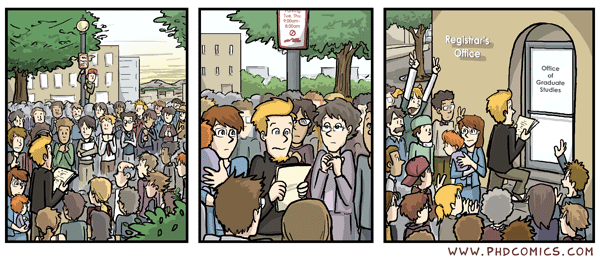
\includegraphics[width=.53\textwidth]{phdcomics-submission02}\par}
\pause{\fontfamily{augie}\small\selectfont PHD Comics by Jorge Cham}\hfill
\includegraphics[width=.53\textwidth]{phdcomics-submission03}

\end{frame}


\begin{frame}
\frametitle{Ever Worried about These?}
\begin{itemize}
\item<2-16> Is my literature survey strong enough?
\item<3-15,17|alert@17|trans:alert@1|handout:alert@1> My bibliography/citation formatting got inconsistent.
\item<4-15,17|alert@17|trans:alert@1|handout:alert@1> My citation and bibliography aren't synchronised!
\item<5-15,17|alert@17|trans:alert@1|handout:alert@1> My math equations don't display/print correctly.
\item<6-16> Should this discussion go under this section or that?
\item<7-15,17|alert@17|trans:alert@1|handout:alert@1> What formatting did I use for my subsection headings again?
\item<8-15,17|alert@17|trans:alert@1|handout:alert@1> Didn't I set that heading to bold and italic 5 minutes ago?
\item<9-15,17|alert@17|trans:alert@1|handout:alert@1> My section/figure/page numbering's gone all wrong!
\item<10-16> Does this subsection go together with this section?
%\item<alert@2> My page numbering's gone all wrong!
\item<11-15,17|alert@17|trans:alert@1|handout:alert@1> Oops, I forgot to update the TOC.
\item<12-16> What results should I put in this table?
%\item<13-16,18|alert@18> How do I fit/split this huge table on/across page(s)?
\item<13-15,17|alert@17|trans:alert@1|handout:alert@1> My figure jumped off the page again!
\item<14-15,17|alert@17|trans:alert@1|handout:alert@1> The application crashed!
\item<15-15,17|alert@17|trans:alert@1|handout:alert@1> \textbf{MY FILE GOT CORRUPTED!!!}
\end{itemize}
\end{frame}

\begin{frame}<1>[label=texNfriends]
\frametitle{What are \TeX\ and \LaTeX,\ and Friends?}

\begin{description}
\item<1>[\TeX] 
\begin{itemize}
\item From Greek $\uptau\upepsilon\upchi$
\item \textsmaller{ASCII} \texttt{TeX}, \textsmaller{\textipa{/tEx/}, \textipa{/tEk/}}
\item A \structure{computer typesetting system} created by Donald Knuth
\item for `the creation of beautiful books'
\end{itemize}


\item<2>[\LaTeX]
\begin{itemize}
\item \textsmaller{ASCII} \texttt{LaTeX}, \textsmaller{\textipa{/"leItEx/}, \textipa{/"leItEk/}, \textipa{/"lA:tEx/}, \textipa{/"lA:tEk/}}
\item A \structure{document preparation system} by Leslie Lamport
	\end{itemize}

\pause

\item<3-4>[Binaries]
	\begin{itemize}
  \item \structure{\hologo{eTeX}}: additional primitives to \hologo{TeX}
	\item \structure{\alert<4>{\hologo{pdfTeX}}}: additional PDF-related primitives
  \item \structure{Xe\TeX}: native UTF-8 input; can access system fonts
	\item \structure{\hologo{LuaTeX}}: includes the Lua scripting engine
\end{itemize}
\item <5>[Friends]
\begin{itemize}
\item \structure{Bib\TeX}, \structure{MakeIndex}, \structure{METAFONT}, \structure{METAPOST},  \ldots
\item \url{http://www.ctan.org/what_is_tex.html}
\end{itemize}
\end{description}
\end{frame}

{\setbeamertemplate{background canvas}{\hskip-2em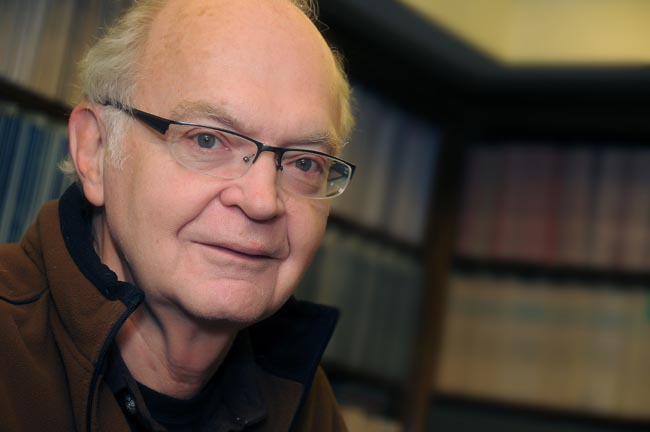
\includegraphics[height=\paperheight]{d_knuth_noticia}}
\setbeamercolor{itemize item}{fg=structure.fg!45}
\begin{frame}[plain,t]
\vfill
\hfill
\begin{minipage}{.42\textwidth}
\usebeamercolor[bg]{normal text}
\hspace{1em}\textbf{\large Donald Knuth (1938--)}
\begin{itemize}
\usebeamercolor[bg]{normal text}
\item American computer scientist, mathematician, and professor emeritus at Stanford University
\item Author of the multi-volume work The Art of Computer Programming
\item ``Father of the analysis of algorithms''
\end{itemize}
\end{minipage}

\bigskip

\begin{quote}
\usebeamercolor[bg]{normal text}
``Science is what we understand well enough to explain to a computer. Art is everything else we do.''

\medskip

``If you optimize everything, you will always be unhappy.''
\end{quote}
\vspace*{-4\baselineskip}\null
\end{frame}}

\mode<beamer>{
  \againframe<2>{texNfriends}
}

{\setbeamertemplate{background canvas}{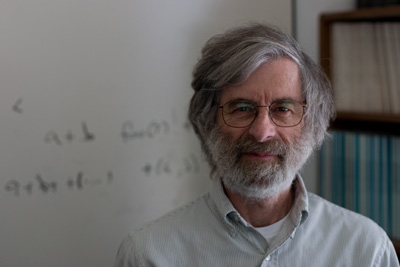
\includegraphics[height=\paperheight]{lamport}}
\setbeamercolor{itemize item}{fg=structure.fg!45}
\begin{frame}[plain,t]
\vfill
\begin{minipage}{.45\textwidth}
\usebeamercolor[bg]{normal text}
\hspace{1em}\textbf{\large Leslie Lamport (1941--)}
\begin{itemize}
\usebeamercolor[bg]{normal text}
\item American computer scientist
\item Laid the foundations of the theory of distributed systems
\end{itemize}

\bigskip

\begin{quote}
\usebeamercolor[bg]{normal text}
``A distributed system is one in which the failure of a computer you didn't even know existed can render your own computer unusable.''\end{quote}
\end{minipage}
\end{frame}
}

\mode<beamer>{
  \againframe<3->{texNfriends}
}

\begin{frame}
\frametitle{Why?}
\framesubtitle{From \url{http://www.ctan.org/what_is_tex.html}}
\begin{columns}[T]
\begin{column}{.46\textwidth}
\begin{block}{Output Quality}
\begin{itemize}
\item It has the best output.
\item It knows typesetting.
\end{itemize}
\end{block}

\begin{block}{Superior Engineering}
\begin{itemize}
\item It's fast.
\item It's stable.
\item It's not rigid (extensible).
\item Plain text input.
\item Many output types.
\end{itemize}
\end{block}
\end{column}

\begin{column}{.46\textwidth}
\begin{block}{Freedom}
\begin{itemize}
\item It's free.
\item It runs anywhere.
\end{itemize}
\end{block}

\begin{block}{Popularity}
\begin{itemize}
\item It's the standard (in academia and science).
\end{itemize}
\end{block}
\end{column}
\end{columns}
\end{frame}

\begin{frame}
\frametitle{Typesetting and Word Processing}
\framesubtitle{Apples and Oranges}
\begin{itemize}
\item<+-> Word processors
\begin{itemize}
\item Replacement of mechanical typewriters
\item Word, OpenOffice, AbiWord, \ldots
\end{itemize}
\item<+-> Typesetting and Desktop publishing
\begin{itemize}
\item For publication and printing
\item InDesign, QuarkXPress, Scribus\ldots
\end{itemize}
\end{itemize}
\end{frame}

\begin{frame}
\frametitle{Scalability}

\centering
\begin{tikzpicture}
%\draw[help lines,gray!20] (0,0) grid (6,4);
%\draw[semithick] (0,0) rectangle (6,4);
\draw[semithick,->,>=latex'] (-.5, 0) -- (6.5, 0);
\draw[semithick,->,>=latex'] (0, -.5) -- (0,5);
\draw[dashed,structure.fg!50!black,semithick] (0, 0.2) parabola (3.5,4) node[above,font=\footnotesize,text=black]{impossible to do} (3.5, 4);
\node[left] at (3,3) {Word$\textsuperscript{\textregistered}$};
\draw[structure.fg!50!black,semithick] (0, 1) parabola (6,3); 
\node at (5.2,2) {\LaTeX};
\node[below,font=\footnotesize] at (3,0) {document complexity and size};
\node[xshift=-8pt,yshift=4pt,font=\footnotesize,transform shape,rotate=90] at (0,2.2) {effort and time consumption};
\end{tikzpicture}

{\small Scalability of \LaTeX\ and Microsoft Word\textregistered\ against document size and complexity (redrawn from Marko Pinteric's original at \url{http://www.pinteric.com/miktex.html})}



\end{frame}

\begin{frame}
\frametitle{Professional Typesetting Quality Output}
\setlength\fboxsep{.25em}

\begin{itemize}
%\item Follows typography best practice
\item<+-> Typesetting quality and legibility
\begin{itemize}
\item good kerning hinting and correct ligatures
\item inter-word, line and paragraph spacing
\item context-sensitive hyphenation
\end{itemize}
%
\begin{columns}[T]
\begin{column}{.48\linewidth}
\fcolorbox{black}{white}{
\begin{minipage}{.98\linewidth}
\centering\large\fontfamily{qtm}\selectfont \alert{Ta}ble \alert{fi}ery \alert{fl}u\alert{ff}y\par
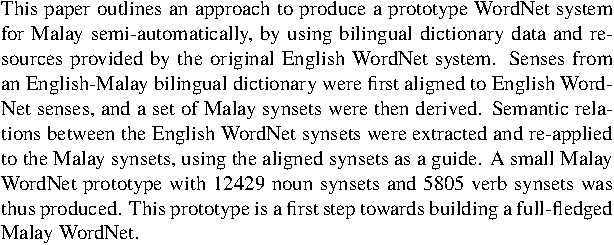
\includegraphics[width=\linewidth]{examples/latex-text-sample}
\end{minipage}}
\end{column}
\begin{column}{.48\linewidth}
\fcolorbox{black}{white}{
\begin{minipage}{.98\linewidth}
\centering\large
\includegraphics[height=.95em]{examples/word-ligature-cropped}\par
\vspace*{-1pt}\onslide<1>{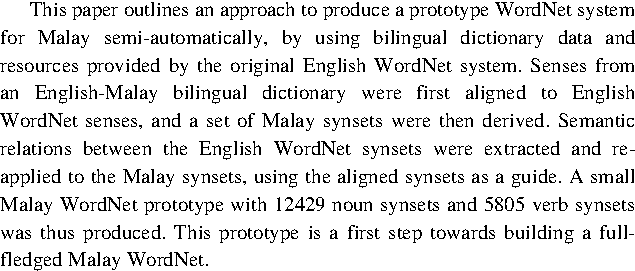
\includegraphics[width=.98\linewidth]{examples/word-text-nohyph-cropped}}\onslide<2-|trans:0|handout:0>{\llap{\setlength\fboxsep{0pt}\colorbox{white}{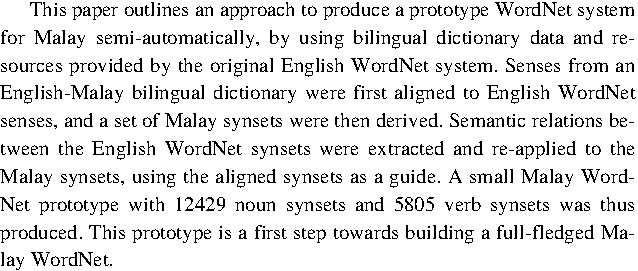
\includegraphics[width=.98\linewidth]{examples/word-text-hyph-cropped}}}}
\end{minipage}}
\end{column}
\end{columns}

\medskip

\item<3-> Correct mathematical typesetting (spacing etc)

\begin{columns}[T]
\begin{column}{.48\linewidth}
\fcolorbox{black}{white}{
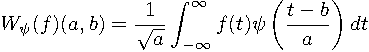
\includegraphics[width=.98\linewidth]{examples/latex-math-sample-cropped}}
\end{column}
\begin{column}{.48\linewidth}
\onslide<3>{\fcolorbox{black}{white}{
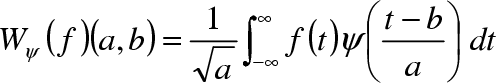
\includegraphics[width=.94\linewidth]{examples/eq-word}}}%
\onslide<4|trans:0|handout:0>{\llap{\fcolorbox{black}{white}{
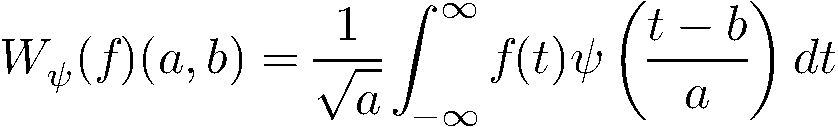
\includegraphics[width=.94\linewidth]{examples/word2010-maths-cropped}}}}
\end{column}
\end{columns}

\end{itemize}
\end{frame}

\begin{frame}
\frametitle{Where Would I Want to Use \hologo{LaTeX}?}
\begin{itemize}
\item Beautiful typographic output \pause(OK not everyone cares that much\ldots)
\item Documents with complex structures
\item Lots of mathematics \pause(or other specific needs)\pause
\item When publishers \alert{require} them
\item Batch processing of data into reports, etc.
\pause
\item Back-end of other applications
\end{itemize}
\end{frame}

%\begin{frame}
%\frametitle{Some Cons}
%\begin{itemize}
%%  \item Usually not WYSIWYG (except commercial solutions)
%  \item Initial learning curve (that's what I'm here for)
%%  \item Hard to produce ``flashy'' docs (with too many fonts, colours\ldots)
%  \item Overkill for simple documents
%  \item Not as suitable for graphic-intensive material (e.g.\ advertising)
%%  \item Not so good for advertisements, etc
%\end{itemize}
%\end{frame}

\begin{frame}
\frametitle{This is not a Word Processors vs \hologo{LaTeX} debate.}
\begin{itemize}
\item It's a `teaser' preview of an alternative tool.
\item Some word processors also provide mechanisms to handle same routine tasks (with varying degrees of ease, consistency and stability)
\item Use the best tool for the task at hand.
\item \textbf{\alert{You}} are the best judge to decide for yourself.
\end{itemize}
\end{frame}


\begin{frame}
\frametitle{How Do I Use It?}
\begin{enumerate}
\item<+-> Write a plain text \hologo{LaTeX} file (\texttt{.tex})
\item<+-> Run it through \texttt{pdflatex} or \texttt{xelatex} $\rightarrow$ \textsmaller{PDF} output\\
\textsmaller{(or \texttt{latex + dvips + ps2pdf} for \textsmaller{DVI} + \textsmaller{PS} + \textsmaller{PDF})}
\item<+-> Run \texttt{bibtex} and/or \texttt{makeindex} to process bibliographies, indices
\item<+-> Re-run \texttt{pdflatex} to resolve references and pointers
\end{enumerate}
\end{frame}

\begin{frame}[fragile]
\frametitle{Example \texttt{.tex} File}
\setlength{\fboxsep}{.5em}

\begin{columns}[T]
\begin{column}{.47\textwidth}
\begin{beamerboxesrounded}[width=\linewidth]{}
\vskip-1.2em
\begin{lstlisting}[moretexcs={maketitle,tableofcontents,subsection},
emph={document,abstract},
basicstyle={\ttfamily\footnotesize\lsstyle},lineskip=-2pt]
\documentclass[a4paper,11pt]{article}
\author{Lim Lian Tze}
\title{An Introductory Paper}
\date{\today}
:\onslide<1-3>{{\bfseries\color{Maroon}\textbackslash usepackage}[\textcolor{Sienna2}{\bfseries english}]\{\textcolor{RoyalBlue3}{\bfseries babel}\}}%
\onslide<4|trans:0|handout:0>{\llap{{\bfseries\color{Maroon}\textbackslash usepackage}[\textcolor{Sienna2}{\bfseries ngerman}]\{\textcolor{RoyalBlue3}{\bfseries babel}\}}}%
\onslide<5|trans:0|handout:0>{\llap{{\bfseries\color{Maroon}\textbackslash usepackage}[\textcolor{Sienna2}{\bfseries bahasam}]\{\textcolor{RoyalBlue3}{\bfseries babel}\}}}:

\begin{document}
\maketitle
\tableofcontents

\begin{abstract}
This paper introduces\ldots
\end{abstract}

\section{Introduction}
We consider\ldots

\section{State of the Art}
We look at\ldots

\subsection{Document Formats}
There are many\ldots
\end{document}
\end{lstlisting}
\vspace*{-1.2em}
\end{beamerboxesrounded}
\end{column}

\begin{column}{.46\textwidth}
\hfill\uncover<3>{\fcolorbox{black}{white}{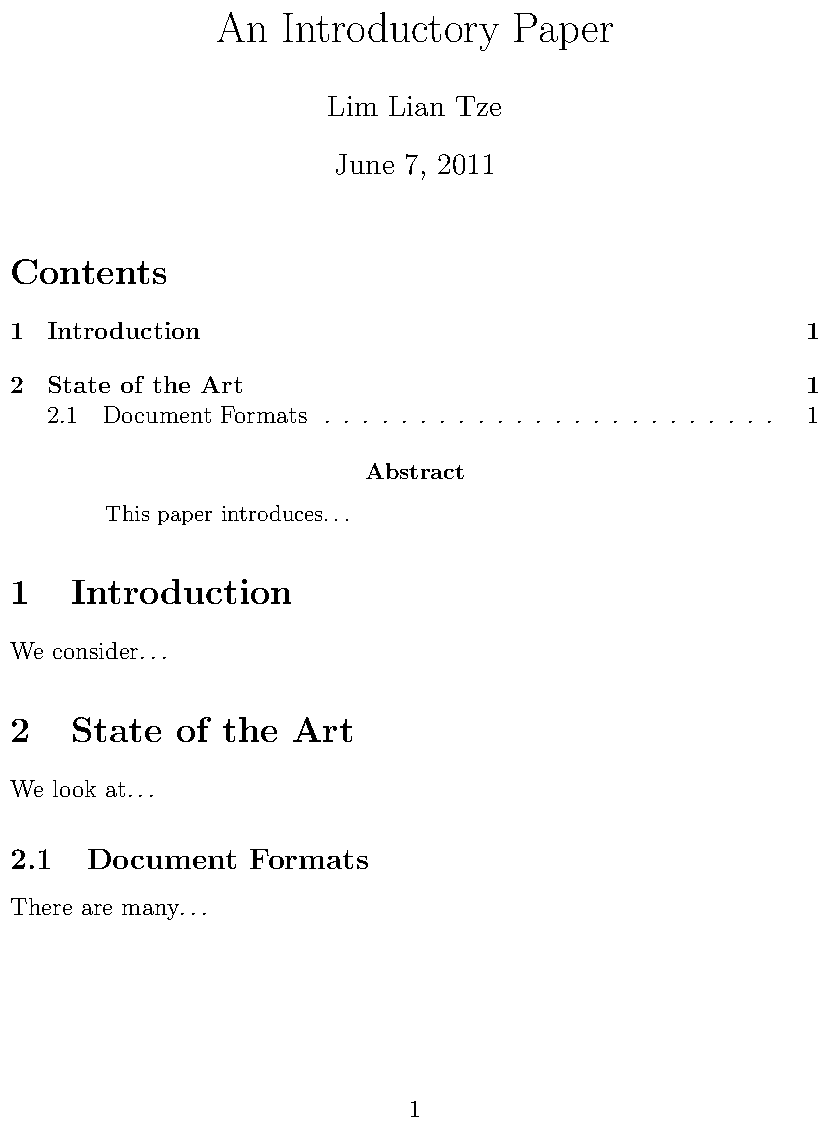
\includegraphics[width=.95\linewidth]{examples/first-en}}}%
\uncover<4|trans:0|handout:0>{\llap{\fcolorbox{black}{white}{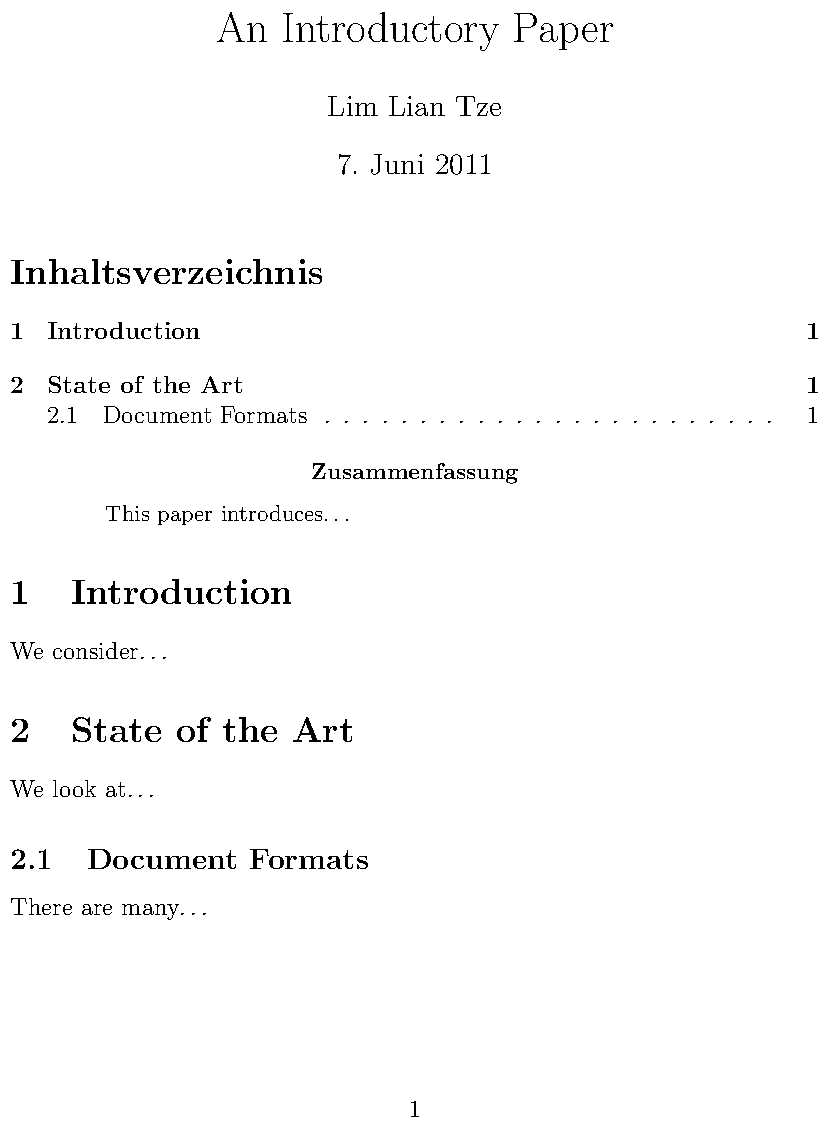
\includegraphics[width=.95\linewidth]{examples/first-de}}}}%
\uncover<5|trans:0|handout:0>{\llap{\fcolorbox{black}{white}{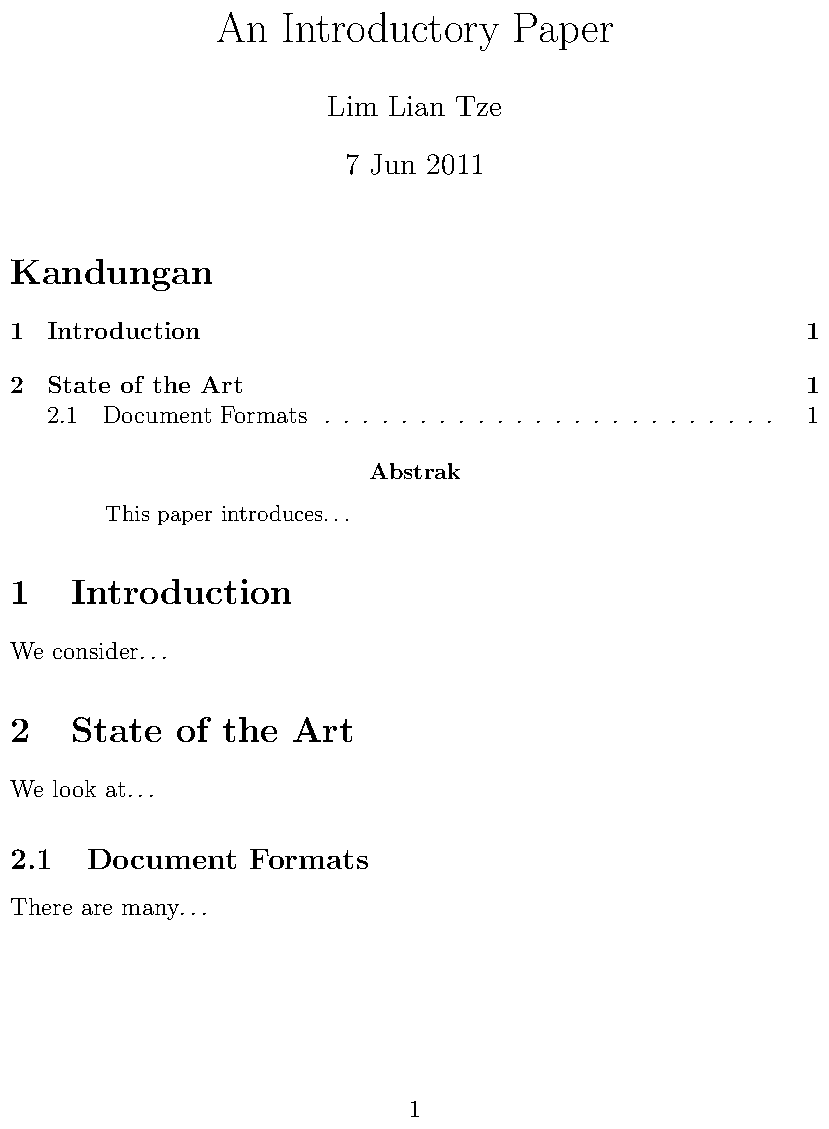
\includegraphics[width=.95\linewidth]{examples/first-ms}}}}
\end{column}
\end{columns}

\uncover<2->{\begin{tikzpicture}[remember picture,overlay]
\node[single arrow,fill=DarkSeaGreen,font=\ttfamily\bfseries,xshift=-1em] at (current page.center) {pdflatex};
\end{tikzpicture}
}

\end{frame}

\begin{frame}
\frametitle{Where Do I Get It?}
\begin{description}
\setlength\labelwidth{8.5em}
\setlength\itemindent{3em}
\item[Online] Overleaf (\url{www.overleaf.com})
\pause
\bigskip
\item[Windows] Mik\TeX, \TeX Live
\item[Un*x, \textsmaller{GNU}/Linux] \TeX Live
\item[Mac OS X] Mac\TeX\ (based on \TeX Live)
\item[Installation] Use your OS' package manager\\\hspace{\itemindent}(or download manually)
\pause
\item[Editors] vi, emacs, Texmaker, TeXworks, Texstudio, TeXshop\ldots
\pause
\item[\hologo{LaTeX} Packages] Use Mik\TeX\ or \TeX Live's package manager
\pause
\bigskip
\item[Documentation] 
{\small (Online)} \url{http://texdoc.net/pkg/<package name>}\\
\hspace{\itemindent}{\small (\TeX Live)} \texttt{\$ texdoc <package name>}\\
\hspace{\itemindent}{\small (Mik\TeX)} \texttt{\$ mthelp <package name>}
\end{description}
\end{frame}

\begin{frame}
\frametitle{Easy to Learn, Hard to Master}
\begin{itemize}
\item<+-> Customising may not be straightforward (vs word processors)
\item<+-> Intentionally so: Style guidelines should be followed strictly
\begin{itemize}
\item Publisher/organisation provides \structure{document class} or \structure{style} files
\item Use these to take care of formatting and styling, focus on the \structure{content}
\end{itemize}
% \item<+-> Fair enough. \\But where do I learn all the stuff the \TeX nicians do?
% \item<+-> (There \emph{is} a learning curve)
\end{itemize}
\end{frame}

\begin{frame}
\frametitle{Too hard, only for engineers/mathematicians?}

\begin{columns}[T]
\begin{column}{0.58\textwidth}
\begin{itemize}[<+->]
\item I once guided a student in the humanities to learn authoring Chinese \LaTeX{} documents entirely through e-mail
\item Recently a 75-year-old user transitioned to \LaTeX{} on Overleaf to write a book (with indices, end notes, cross references)
\item Professor in Finance at Trinity College transitioned to \LaTeX{} successfully (\url{https://www.overleaf.com/blog/299})
\item Linguists, psychologists, biostatistics (integrating with R), legal profession\ldots
\end{itemize}
\end{column}
\hfill
\begin{column}{.29\textwidth}<3->
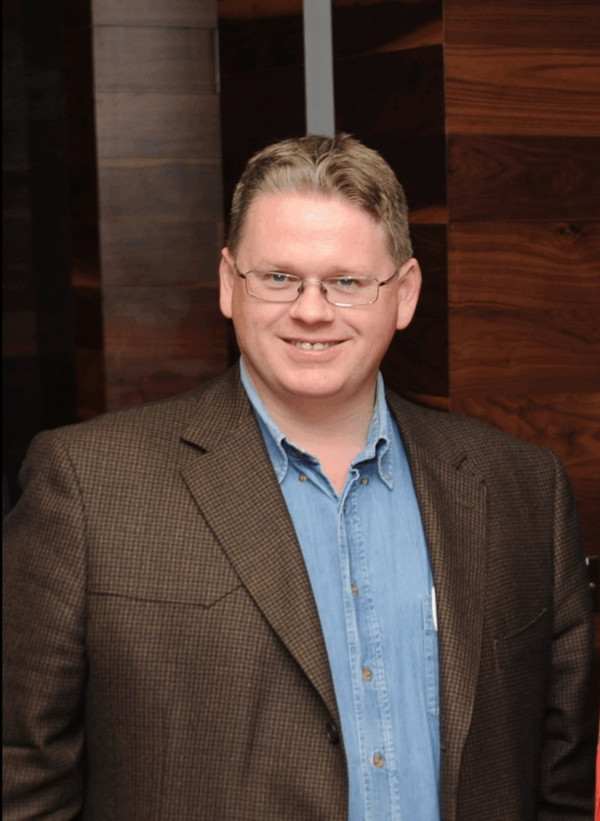
\includegraphics[width=\linewidth]{brian-lucey-full}\\
{\footnotesize Prof Brian Lucey, Trinity College, Dublin}
\end{column}
\end{columns}

\end{frame}

{\setbeamertemplate{background canvas}{\hskip-1.75em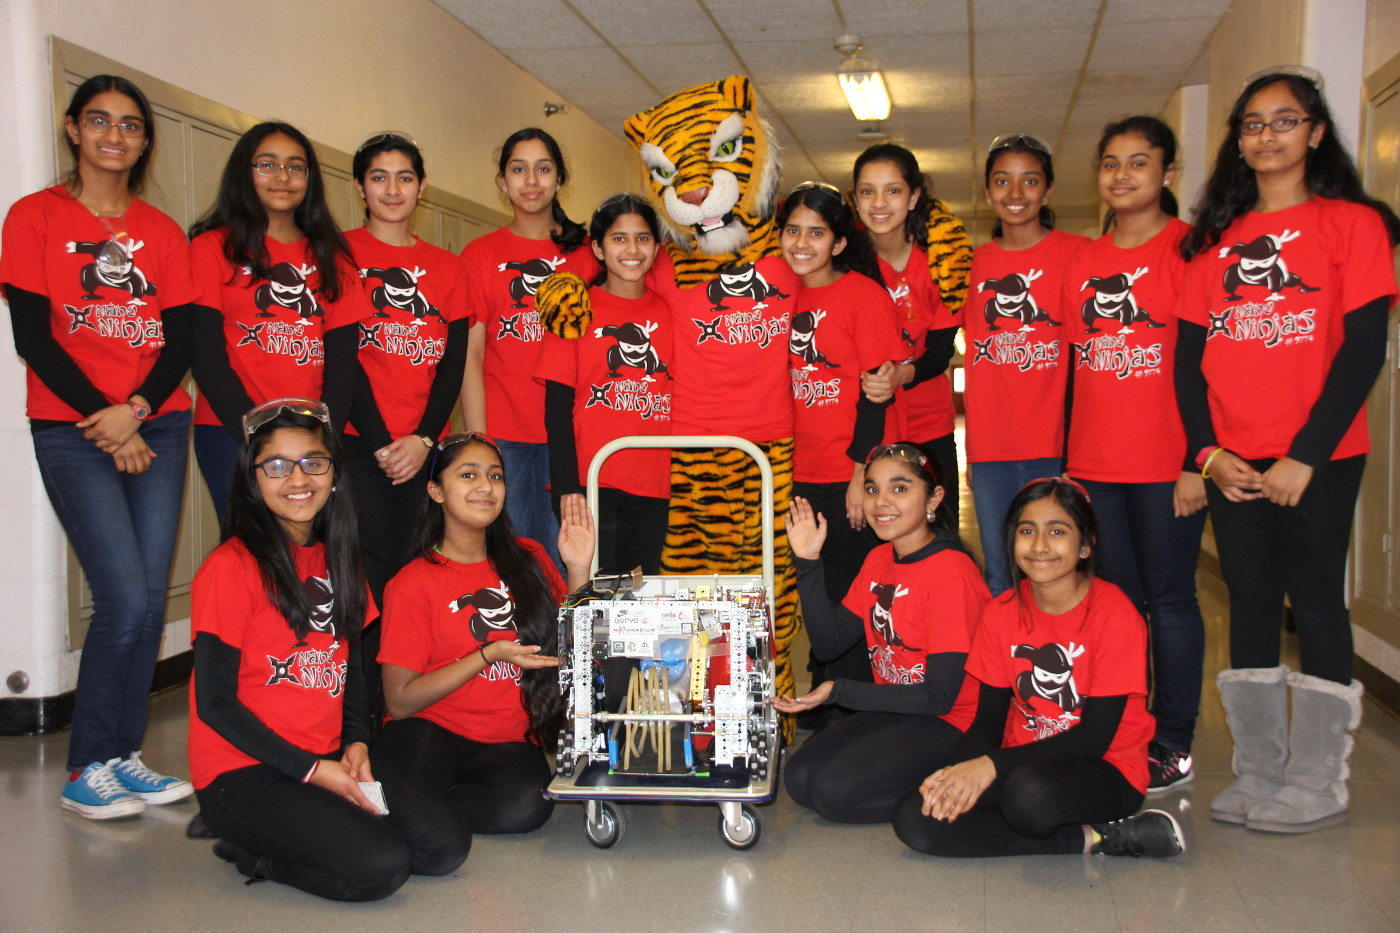
\includegraphics[height=\paperheight]{IMG_1710}}
\begin{frame}[plain,t]
\tikz\node[text=palette tertiary.fg,fill=palette tertiary.bg,opacity=0.8,font=\small\bfseries,text width=\textwidth,align=center]{Nano Ninjas -- a group of 7th- and 8th-graders from Portland, OR};

\vspace*{.87\textheight}

\tikz\node[text=palette tertiary.fg,fill=palette tertiary.bg,opacity=0.8,font=\footnotesize,text width=\textwidth,align=center]{Collaboratively wrote an engineering notebook with \textbf{300+ pages} in \LaTeX{} as part of their FIRST Tech Challenge win (\url{https://www.overleaf.com/read/hkxzqcncngyv})};
\end{frame}
}

\begin{frame}
\centering\Huge
So, What Can \hologo{LaTeX} Do?
\par
\end{frame}
        \begin{frame}
            \frametitle{Contents}
            \tableofcontents
        \end{frame}
    \section{Control policies in epidemics}
        {
\begin{frame}{Control policies}
    \begin{textblock*}{55mm}(2mm, 10mm)
        \begin{beamerboxesrounded}{Optimal control theory is a way.}
            \begin{itemize}
                \item \only<2->{
                    We require a \textbf{model} to describe the spreading of an 
                    uncontrolled disease, and whose transitions generate a 
                    \textbf{cost or reward}.
                    }
                \item \only<3->{
                    Continuous \textbf{control action} that modify changes 
                    between states.
                    }
                \item \only<4->{
                    A \textbf{functional} which describes \textbf{cost-reward}.
                    }
            \end{itemize}
        \end{beamerboxesrounded}
    \end{textblock*}
%
    \begin{textblock*}{65mm}(62mm, 10mm)
        \begin{beamerboxesrounded}{Control Policy}
            \begin{itemize}
                \item \only<5->{
                    A rule that prescribes which control
                    operation to use at each time, is a \textbf{control policy}.
                }
                \item \only<6->{
                    \textbf{closed-loop} or \textbf{feedback} control.
                }
                \item \only<7->{
                    \textbf{open-loop} policy.
                }
            \end{itemize}
            %
            \only<8>{
                We consider control policies that affect the bounded rates at which 
                population moves from one class (e.g., infected) to another (e.g., 
                recovered).
            }
        \end{beamerboxesrounded}
    \end{textblock*}
    %
    %
    \begin{textblock*}{90mm}(25mm, 65mm)
        \begin{bibunit}[apalike]
            \nocite{Wickwire1977}
            \putbib
        \end{bibunit}
    \end{textblock*}
\end{frame}
}
        \begin{frame}{SARS: isolation and quarantine}
    \only<1-4>{
    \begin{textblock*}{55mm}(2mm, 12mm)
            If an disease lacks of a rapid diagnostic test, therapy or 
        vaccine, then isolation and quarantine .
%
            Gumel et. al %\cite{Gumel2004}
            model this strategies for (SARS).
    \end{textblock*}
    }
%        
    \only<2-4>{
    \begin{textblock*}{55mm}(65mm, 12mm)
            Based in the work of Gumel et. al., Yan and Zou report 
            %\cite{Yan2008} 
            a control epidemic model for SARS. They use 
            quarantine and isolation as mitigation controls. 
     \end{textblock*}
    }
%
%
    \only<4-6>{
    \begin{textblock*}{65mm}(17mm, 35mm)
     \begin{equation*}\label{eqn:sars_model}
        \begin{aligned}
            \dfrac{dS}{dt} &=
                \Lambda 
                -\dfrac{
                    S
                    \left(
                        \beta I 
                        + \mathcal{E}_E  \beta E
                        + \mathcal{E}_Q  \beta Q
                        + \mathcal{E}_J  \beta J
                    \right)
                }{N}
                - \mu S,
            \\
            \dfrac{dE}{dt} &=
                p +
                \dfrac{
                    \beta S
                    \left(
                        \beta I 
                            + \mathcal{E}_E \beta E
                            + \mathcal{E}_Q \beta Q
                            + \mathcal{E}_J \beta J
                    \right)
                }
                {N}
                -(
                \only<5->{
                    \textcolor{cyan}{u_1(t)}
                }
                     + k_1 + \mu
                )E,
            \\
            \dfrac{dQ}{dt} &=
                \only<5->{
                    \textcolor{cyan}{u_1(t)}
                }
                 E - (k_2 + \mu) Q,
            \\
            \dfrac{dI}{dt} &=
                k_1 E 
                -(
                \only<5->{
                    \textcolor{cyan}{u_2(t)}
                }
                + d_1  + \sigma_1 + \mu) I,
            \\
            \dfrac{dJ}{dt} &=
                \only<5->{
                    \textcolor{cyan}{u_2(t)}
                }
                  I 
                + k_2 Q
                - (d_2 + \sigma_2 + \mu) J,
            \\
            \dfrac{dR}{dt} &=
                \sigma_1 I
                +\sigma_2 J
                - \mu R.
        \end{aligned}
     \end{equation*}
    \end{textblock*}
    }
    \only<5-6>{
        \begin{textblock*}{55mm}(15mm, 12mm)
            \begin{equation*}\label{eqn:sars_cost}
              \min_{u \in U}\int_{0}^{t_f}
                  \left[
                    B_1 E(t)
                    + B_2 Q(t)
                    + B_3 I(t)
                    + B_4 J(t)
                    + \frac{C_1}{2} u_1^2 (t)
                    + \frac{C_2}{2} u_2^2 (t)
                  \right]
                  dt.
            \end{equation*}
        \end{textblock*}
    }
    
\end{frame}
    \section{Existence and characterization of optimal policies}
        \begin{frame}{Existence and characterization of optimal policies}
    \only<1>{
    \begin{textblock*}{100mm}(15mm, 12mm)
        The non controlled epidemic model described above is of the
        form 
        \begin{eqnarray*}
            \dot{X} & = & AX +  
            \begin{bmatrix}
                X^\top B^{(1)}\\
                \vdots \\
                X^\top B^{(n)}
            \end{bmatrix}X + k  \\
            & = & \left(A + [X^\top \cdots X ^ \top]
            \begin{bmatrix}
                    B^{(1)}\\
                    \vdots \\
                    B^{(n)}
            \end{bmatrix} \right) X + k
        \end{eqnarray*}
        where the matrix $A$ represents the linear part of the system, each 
        matrix $B^{(j)}$, $j=1,\ldots,n$, 
        gives the {\it interaction} part as a quadratic 
        form, and $k$ is a constant vector.
        
         Thus the $j$-th row of the above system takes the form 
            \[ \dot{X}_j = r_j(A)X + X^\top B^{(j)}X + k_j.\]
    \end{textblock*}
    }
\end{frame}
%
%
%
\begin{frame}{A family of control systems}
    Let $\mathbf{X} \subset \mathbb{R} ^ n$ and 
    $\mathbf{U} \subset \R^m$ be nonempty 
    and compact sets. The sets $\mathbf{X}$ and $\mathbf{U}$ are 
    respectively called the {\it state space} and the {\it control space}. The 
    vectors in $X$ have non-negative entries, in particular we assume that 
    $0\in X$. The control set $\mathbf{U}$ is convex. We consider the following 
    control system, for $j=1,\ldots,n$, 
    \begin{equation*}
        \dot{X}_j  =  [r_j(A) + u^\top C^{(j)}]X +
        X^\top    \begin{bmatrix}
        r_1(B^{(j)}) + u^\top D^{(j1)}\\
        \vdots \\
        r_n(B^{(j)}) + u^\top D^{(jn)}
      \end{bmatrix}  X + k_j
    \end{equation*}
    where $A\in\R^{n\times n}$,
    $B^{(j)}\in\R^{n\times n}$, 
    $C^{(j)}\in\R^{m\times n}$,
    and $ D^{(jl)}\in\R^{m\times n}$ for $l=1,\ldots,n$.
\end{frame}
%
%
%
%
\begin{frame}{}
    \begin{equation*}
        \dot{X}_j  =  [r_j(A) + u^\top C^{(j)}]X +
        X^\top    \begin{bmatrix}
        r_1(B^{(j)}) + u^\top D^{(j1)}\\
        \vdots \\
        r_n(B^{(j)}) + u^\top D^{(jn)}
      \end{bmatrix}  X + k_j, \quad j=1,\dots, n.
    \end{equation*}
%
    \begin{theorem}
        For each measurable function 
        $u:[0,T]\to \mathbf{U}$ and each initial condition $x_0\in X$,
        there exists a unique absolutely continuous function 
        $X_u:[0,T]\to \R^n$ that satisfies the the 
        system  almost everywhere. 
    \end{theorem}
\end{frame}
%
%
%
\begin{frame}{Existence of optimal policies.}
    Consider the  {\it cost functional} of an admissible control $u$, given the 
    initial state $x_0$, 
    \begin{equation}\label{CostFunctional} 
        V(u,x_0) := \int_0 ^ T g(X(t), u(t)) \ ,dt,
    \end{equation}
    %
    where $g: \mathbf{X} \times \mathbf{U} \to \R$ is continuous. 
    The {\it optimal control problem} (OCP) consists of finding an admissible 
    control $u^\ast$ such that
    \[ V(u^\ast,x_0)=\inf\{ V(u,x_0)\mid u\in \mathbb{U}_B \}.\]
    If there exists such a control $u^\ast$, then it is called an 
    {\it optimal policy} or {\it optimal control}. 
    The pair $(u^\ast,X^\ast)$, where $X^\ast$ is given by 
    the above Theorem, is an {\it optimal pair}.
\end{frame}

        \begin{frame}{Sufficient conditions for optimality}
    Consider the Hamiltonian 
    $
        \mathcal{H}:\mathbf{X}\times\mathbf{U}\times\R^n\to \R
    $, defined as 
    \[
        \mathcal{H}(x, u, \lambda):=
             g(x,u) + \lambda ^ \top f(x,u),
    \]
        and
        \[ 
            \mathcal{H}^\ast(x,\lambda)  
            := \inf_{u\in\mathbf{U}}\mathcal{H}(x,u,\lambda),
        \]
        where $g$ determines the cost functional 
        and $f$ is given by the right-hand side of the control system.

        The function $\lambda:[0,T]\to \R^n$ and the admissible pair 
        $(u,X)$ satisfy the necessary conditions of the 
        {\it Maximum Principle} (MP) if they solves
        {\it adjoint equation}
        \begin{equation*}
             \dot{\lambda}(t) = -\mathcal{H}_x(X(t),u(t),\lambda(t))^\top, 
             \quad \lambda(T)=0,
        \end{equation*}
        and satisfy the {\it optimality condition}
        \begin{equation*}\label{OptCond}
            \mathcal{H}^\ast(X(t),\lambda(t)) =
            \mathcal{H}(X(t),u(t),\lambda(t)).
       \end{equation*}
\end{frame}

\begin{frame}{}
    \begin{definition}\label{PiecewiseCont}
        \rm The function $w$ from $[0,T]$ to some Euclidean space is {\it 
        piecewise continuous} if
        \begin{enumerate}[(i)]
            \item $w$ is continuous on $[0,T]$ except at a finite number of 
            points, and 
            \item if $w$ is discontinuous at $t$, then  
                \[\lim_{s\to t^-}w(s) \mbox{ and } \lim_{s\to t^+}w(s)\]
                are finite. 
        \end{enumerate}
    \end{definition}
\end{frame}

\begin{frame}{Pontryagin MP}
    \begin{textblock*}{60mm}(1mm, 10mm)
        \begin{beamerboxesrounded}{Optimality condition}
            \begin{equation*}
                \begin{aligned}
                    \mathcal{H}(x,u,\lambda)
                        &:= g(x,u) + \lambda^\top f(x,u),
                    \\
                    \mathcal{H}^\ast(x,\lambda)  
                        &:= \inf_{u\in\mathbf{U}}\mathcal{H}(x,u,\lambda),
                    \\
                    \mathcal{H}^\ast(X(t),\lambda(t)) 
                        &=
                    \mathcal{H}(X(t),u(t),\lambda(t)).
                    \\
                \end{aligned}
            \end{equation*}
        \end{beamerboxesrounded}
    \end{textblock*}
    
    \begin{textblock*}{60mm}(65mm, 10mm)
        \begin{beamerboxesrounded}{adjoint equation}
            \begin{align*}
                 \dot{\lambda}(t) &= -\mathcal{H}_x(X(t),u(t),\lambda(t))^\top, 
                 \\
                 \quad \lambda(T) &=0.
            \end{align*}
        \end{beamerboxesrounded}
    \end{textblock*}
%
%
%
%
    \begin{textblock*}{120mm}(5mm, 40mm)
        \begin{theorem} 
            Let $\lambda:[0,T]\to \R^n$  be a continuous function 
            and let $(u^\ast,X^\ast)$ be an admissible pair such that 
            \begin{enumerate}[\rm (i)]
                \item 
                    $u^\ast$ is piecewise continuous,
                \item 
                    $\dot{X}^\ast$ exists and is piecewise continuous,
                \item 
                    $(\lambda,u^\ast,X^\ast)$ satisfies the optimality 
                    condition, and,
                \item 
                    except at the points of discontinuity of $u^\ast$, the 
                    adjoint equation holds.
            \end{enumerate}
            If, for each $t$, the function $\mathcal{H}^\ast(\cdot,\lambda(t))$ 
            is convex on $\mathbf{X}$, then $(u^\ast,X^\ast)$ is an optimal
            pair.
        \end{theorem}
    \end{textblock*}
\end{frame}

\begin{frame}{Example HIV }
    \begin{textblock*}{120mm}(1mm, 11mm)
        Consider the uncontrolled HIV model  reported in 
        (Butler 1997)
        \begin{align*}
            \dfrac{dT}{dt} &= \dfrac{s}{1 + V} - \mu_{1}T + rT \left( 1 - %
                                \dfrac{T + T_{i}}{T_{max}} \right) 
                                - 
                                \only<3->{
                                    \textcolor{cyan}{u(t)}
                                }
                                k_{1} V T 
            \\
            \dfrac{dT_{i}}{dt} &= 
                \only<3->{
                    \textcolor{cyan}{u(t)}
                }
                k_{1}VT - \mu_{2}T_{i} 
                \only<4->{
                    \tag{$\star$}
                }
            \\
            \dfrac{dV}{dt} &= N \mu_2 T_{i} - \mu_{3}V
        \end{align*}
    \end{textblock*}
    \begin{textblock*}{90mm}(5mm, 67mm) 
        \only<1>{
        \begin{bibunit}[apalike]
            \nocite{butler1997optimal}
            \putbib
        \end{bibunit}
        }
        \only<2->{
            If $u(t)$ describes a treatment which modifies the $T$-cells,
        }    
        \only<4->{
            then the problem reads
            $$
                \max_{u} 
                \int_{t_i}^{t_f} {
                    \left[ AT(t) - 
                     (1 - u(t))^{2} \right]
                     } dt, 
            $$
            subject to ($\star$).
        }
    \end{textblock*}
    \only<5>{
    \begin{textblock*}{68mm}(55mm, 35mm)
        \begin{beamerboxesrounded}{
        $
            H(t,x,u,\lambda) 
            = AT - (1 - u)^{2} + \left<\lambda, f \right> 
        $, \qquad
        $\dot{\lambda}(t) = -\mathcal{H}_x(X(t),u(t),\lambda(t))^\top$,
        $\lambda(T)=0$
        }
            \begin{align*}
                \dot{\lambda}_{T}   
                    &=  - A + \lambda_{T} \left[\mu_1 
                    - r\left(1 - \dfrac{T_i}{T_{max}}\right) \right] - 
                    \lambda_{T_i} u k V
                    \\ 
                \dot{\lambda}_{T_i} &=  \lambda_{T}\dfrac{rT}{T_{max}} + 
                    \lambda_{T_i}\mu_2 - \lambda_{V}N\mu_2
                    \\
                \dot{\lambda}_{V}   &=  \lambda_{T} \left(\dfrac{s}{(1+V)^2} + 
                    u k T\right) - \lambda_{T_i}ukT + \lambda_{V}\mu_{3}
            \end{align*}
        \end{beamerboxesrounded}
    \end{textblock*}
    }
\end{frame}
    \section{Numerical analysis}
    	\begin{frame}{Indirect Methods}
	Since we can transform the problem of optimal control into the two-point 
	boundary ODE problem:
	\begin{equation*}
		\label{eqn:extended_tpvbp}
		\begin{aligned}
			\dot{x}(t) &= 
				f(x(t), u(t)), \qquad x(0)=x_0 
			\\
			\dot{\lambda}(t) &=
				-\mathcal{H}_x(x(t),u(t),\lambda(t))^\top, \quad 
				\lambda(T)=0
		\end{aligned}
	\end{equation*}
	methods designed to solve boundary value problem are applicable.
\end{frame}
%
\begin{frame}{The most popular}
    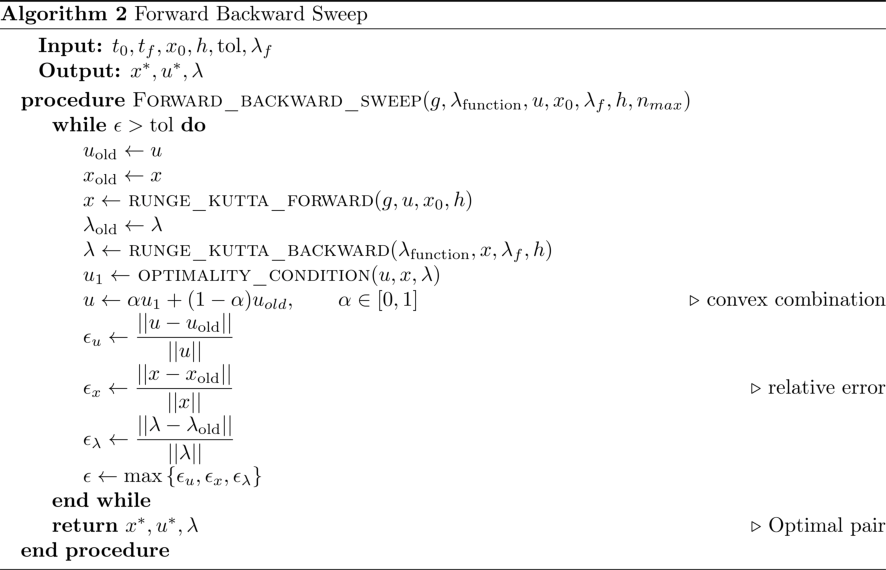
\includegraphics[width=1\linewidth]{fbs_algorithm}
\end{frame}
        \begin{frame}{SARS: isolation and quarantine}

    \begin{textblock*}{65mm}(17mm, 35mm)
     \begin{equation*}\label{eqn:sars_model}
        \begin{aligned}
            \dfrac{dS}{dt} &=
                \Lambda 
                -\dfrac{
                    S
                    \left(
                        \beta I 
                        + \mathcal{E}_E  \beta E
                        + \mathcal{E}_Q  \beta Q
                        + \mathcal{E}_J  \beta J
                    \right)
                }{N}
                - \mu S,
            \\
            \dfrac{dE}{dt} &=
                p +
                \dfrac{
                    \beta S
                    \left(
                        \beta I 
                            + \mathcal{E}_E \beta E
                            + \mathcal{E}_Q \beta Q
                            + \mathcal{E}_J \beta J
                    \right)
                }
                {N}
                -(
                    \textcolor{cyan}{u_1(t)}
                     + k_1 + \mu
                )E,
            \\
            \dfrac{dQ}{dt} &=
                 \textcolor{cyan}{u_1(t)}
                 E - (k_2 + \mu) Q,
            \\
            \dfrac{dI}{dt} &=
                k_1 E 
                -(
                    \textcolor{cyan}{u_2(t)}
                + d_1  + \sigma_1 + \mu) I,
            \\
            \dfrac{dJ}{dt} &=
                    \textcolor{cyan}{u_2(t)}
                  I 
                + k_2 Q
                - (d_2 + \sigma_2 + \mu) J,
            \\
            \dfrac{dR}{dt} &=
                \sigma_1 I
                +\sigma_2 J
                - \mu R.
        \end{aligned}
     \end{equation*}
    \end{textblock*}
        
    \begin{textblock*}{55mm}(15mm, 12mm)
            \begin{equation*}\label{eqn:sars_cost}
              \min_{u \in U}\int_{0}^{t_f}
                  \left[
                    B_1 E(t)
                    + B_2 Q(t)
                    + B_3 I(t)
                    + B_4 J(t)
                    + \frac{C_1}{2} u_1^2 (t)
                    + \frac{C_2}{2} u_2^2 (t)
                  \right]
                  dt.
            \end{equation*}
    \end{textblock*}
\end{frame}

\begin{frame}{}
    \begin{table}
        \begin{center}
            \begin{tabular}{@{}rlrl@{}}
                \toprule
                \multicolumn{4}{c}{\bf{Parameters values}}
                \\
                \midrule
                $\beta$
                & \num{0.2}
                & $d_1$, $d_2$
                & \num{0.0079}, \num{0.0337}
                \\
                $\varepsilon_E$, 
                $\varepsilon_Q$,
                $\varepsilon_J$
                & \num{0.3}, \num{0.0}, \num{0.1}
                &
                $k_1$, $k_2$ 
                & 
                \num{0.1},
                \num{0.125}
                \\
                $\mu$
                & \num{0.000034}
                \\
                $\Lambda$
                & $\mu N$
                \\
                $p$
                & \num{0.0}
                \\
                $\sigma_1$, $\sigma_2$
                & \num{0.0337}, \num{0.0386}
                && \multicolumn{1}{c}{\bf{Initial conditions}}
                \\
                \cmidrule{4-4}
                &&& $S(0)=\num{12e6}$, $E(0)=1565$,
                \\
                $t_f$
                & $\SI{1.0}{year}$
                && $Q(0)=292$, $I(0)=\num{695}$,
                \\
                Step size
                & $dt=\SI{1.0}{day}$
                && $J(0)=\num{326}$, $R(0)=\num{20}$
                \\
                $u_i$ bounds
                & \num{.05}, \num{0.5}
                \\
                $B_1$, $B_2$, $B_3$, $B_4$
                & \num{1.0}, \num{1.0}, \num{1.0}, \num{1.0}
                \\
                $C_1$, $C_2$
                & \num{300}, \num{600}
                \\
                \bottomrule
            \end{tabular}
        \end{center}
    \end{table}
\end{frame}

\begin{frame}{}
    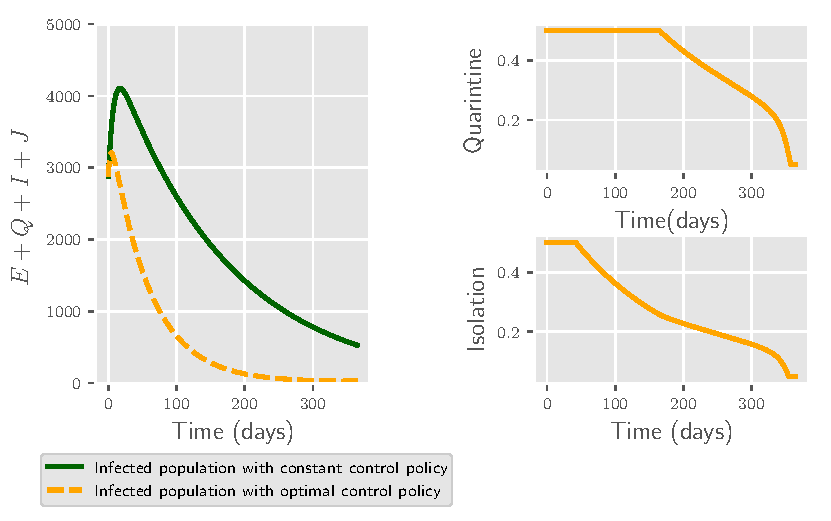
\includegraphics[width=\linewidth]{figure_1_sars-eps-converted-to.pdf}
\end{frame}
\begin{frame}{}
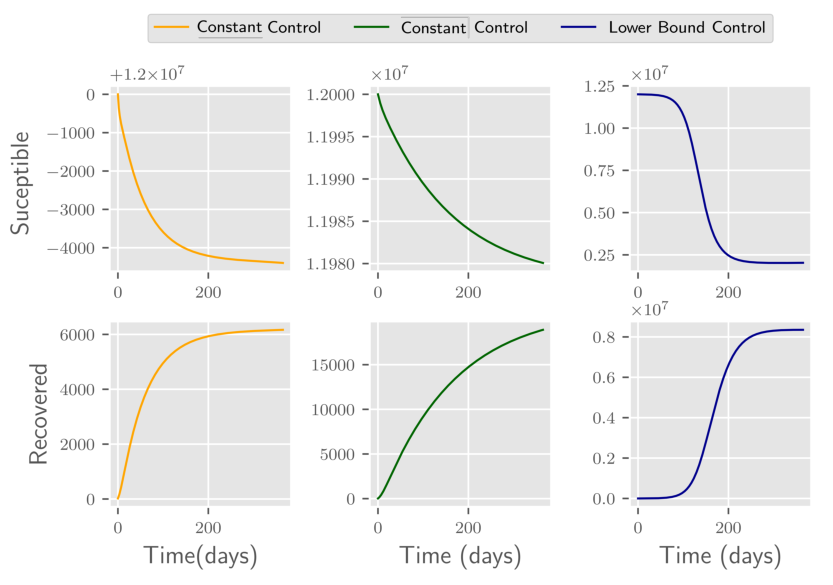
\includegraphics[width=\linewidth]{figure_2_sars-eps-converted-to.pdf}
\end{frame}
\begin{frame}{}
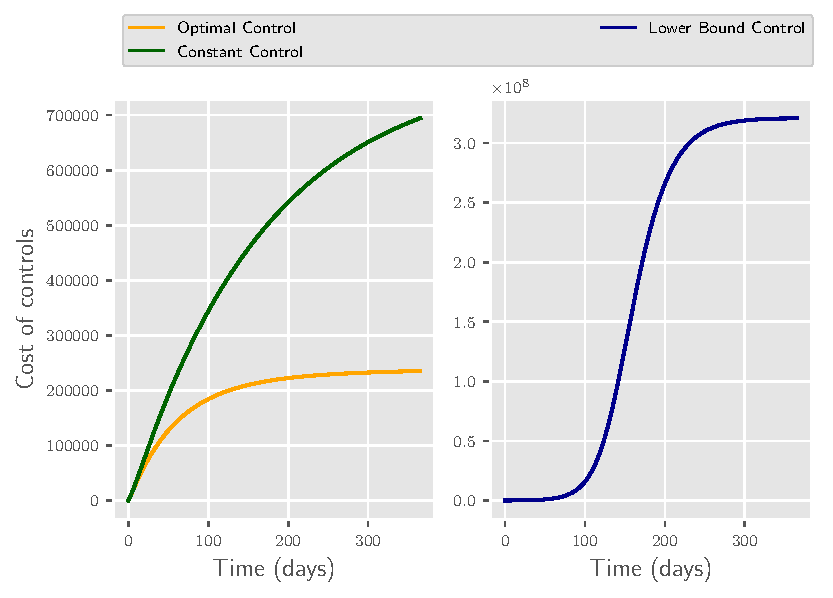
\includegraphics[width=\linewidth]{figure_3_sars-eps-converted-to.pdf}
\end{frame}
    \section{Concluding remarks}
        \begin{frame}{Concluding remarks}
    
    {\bf Uniqueness of optimal policy}.
    The proof of the uniqueness of the state path $X_u$, given a policy $u$, is
    fairly standard. However, the uniqueness of an 
    {\it optimal policy} is not trivial and it can be established on some small 
    enough interval.
    
    {\bf Numerical schemes.}
    According with the forward-backward-sweep, the 
    schemes needs a ODE solver one of its steps. However some times this solver 
    generates spurious solutions as resulting of numeric instability. 
    We see an opportunity to  apply nonstandard numerical schemes which are consistent with 
    the underlying conservation laws.
    
    Direct methods
\end{frame}
\begin{frame}{}
    
    {\bf Maximum principle vs. Dynamic programming.} 
    The same approach is followed in almost all the related literature on optimal
    control of epidemics/diseases.
    
     As an alternative, the so-called Dynamic
    programming approach can be used to analyze this kind of problems. With the
    Maximum principle we need to solve a system of ordinary differential equations
    (ODEs) whereas in Dynamic programming a partial differential equation (PDE)
    arises. In addition, both approaches involve an optimization problem. 
        
    By following the DP approach, the optimal policies are obtained in {\it feedback} (or {\it Markov}) form, i.e., the control policy is a function of the state of the system. Thus DP is a natural approach to solve stochastic models.
\end{frame}
    \begin{frame}{References}
    Complete list of references:
    \href{https://www.overleaf.com/read/vnvgjdqkmznc%
    }{https://www.overleaf.com/read/vnvgjdqkmznc}
    
    Python code:
    \nocite{python_repo}
    \bibliographystyle{amsalpha}
    \bibliography{references.bib}
\end{frame}
\end{document}
